% ****** Start of file template-FFR120-FYM120-blindtext.tex ******
%
% use on Overleaf!!!!
%
\documentclass[%
 reprint,
 amsmath,amssymb,
 aps,
]{revtex4-2}

\usepackage{graphicx}% Include figure files
\usepackage{dcolumn}% Align table columns on decimal point
\usepackage{bm}% bold math
\usepackage{hyperref}% add hypertext capabilities
%\usepackage[mathlines]{lineno}% Enable numbering of text and display math
%\linenumbers\relax % Commence numbering lines
\usepackage{xcolor}
\usepackage{tikz}
\usetikzlibrary{arrows.meta,positioning,shapes.geometric}

\usepackage{lipsum}
\usepackage{array}
\usepackage{ltablex}

\begin{document}

\title{[L] Clogging in Granular Flor through a Bottleneck}% Force line breaks with \\

\author{Marnick Huisman [}
\author{César Mejía ]}

\date{\today}% It is always \today, today,
             %  but any date may be explicitly specified
\begin{abstract} %%% DO NOT CHANGE!
%%% - B1 - %%%%%%%%%%%%%%%%%%%%%%%%%%%%%%%%%%% 
%%% Customize this part: text between - B1 - and - E1 - must not appear in the final report 
 \noindent This project investigates clogging phenomena in granular flows through a bottleneck. We aim to quantify how the probability of clogging and the statistics of particle discharge depend on the orifice diameter, grain size distribution, and particle-wall friction. We will explore a combination of molecular dynamics simulations and cellular automata models to capture both realistic contact interactions and rapid parameter sweeps. The study will provide insights into the mechanisms behind the formation of archs and flow interruptions in granular materials.
 
%%% - E1 - %%%%%%%%%%%%%%%%%%%%%%%%%%%%%%%%%%%%%%

\begin{description} %%% DO NOT CHANGE!
\item[Project Topic] %%% DO NOT CHANGE!
{Granular Matter} %CHANGE accordingly
\item[Teaching Assistant] %%% DO NOT CHANGE!
{Agnese Callegari} % CHANGE accordingly
\end{description} %%% DO NOT CHANGE!
\end{abstract}

\maketitle




\section{\label{sec:intro}Introduction} %%% DO NOT CHANGE!

%%% - B2 - %%%%%%%%%%%%%%%%%%%%%%%%%%%%%%%%%%% 
%%% Customize this part: text between - B2 - and - E2 - must not appear in the final report 
\noindent Granular flows through constrictions occur in many industrial and natural processes, such as hopper discharges, pedestrian evacuations, granular silo flows or even sand clocks. A key feature of these systems is the formation of arches that block flow, known as clogging. Understanding the statistical properties of clogging, including how it depends on particle and system parameters, is important for optimizing material handling and predicting jamming events. Previous work has shown that orifice size, particle size distribution, and frictional properties significantly affect clogging probability. In this project, we will try to model these effects using computational methods and look at the results to see what patterns appear. Some simpler models might not capture all the details, but they can still give a useful idea of how clogging behaves in different situations. The goal is to get a better sense of which parameters are most relevant for clogging and how they interact.

%%% - E2 - %%%%%%%%%%%%%%%%%%%%%%%%%%%%%%%%%%%%%%

\section{\label{sec:overview}Overview} %%% DO NOT CHANGE!

%%% - B3 - %%%%%%%%%%%%%%%%%%%%%%%%%%%%%%%%%%% 
%%% Customize this part: text between - B3 - and - E3 - must not appear in the final report 


\noindent To study clogging, several computational methods are available. \textbf{Table~\ref{tab:methodsoverview}} summarizes three relevant approaches, detailing their use case, key features, and suitability for the project.\\

\begin{table*}[htb]
\centering
\caption{\textbf{Overview of Simulation Methods/Models for Granular Flow Clogging.}}
\label{tab:methodsoverview}

    \begin{tabular}{|c|c|c|c|}
    \hline
    \textbf{Method / Model} &
    \textbf{Use Case Scenario} &
    \textbf{Key Features (Summary)} &
    \textbf{Suitable for the Project?} \\
    \hline
    
    \raisebox{0pt}[3em][3em]{\shortstack[c]{Molecular Dynamics /\\Particle Simulations}} &
    \shortstack[c]{Simulating individual grains in\\hopper or bottleneck flows} &
    \shortstack[c]{\vspace{5pt}\\Resolves particle contacts, friction\\and normal forces, realistic arch\\formation; computationally intensive\\for large systems} &
    \raisebox{0pt}[3em][3em]{\shortstack[c]{\textbf{Yes} — main method to\\reproduce realistic\\clogging dynamics.}}\\
    \hline
    
    \raisebox{0pt}[3em][3em]{\shortstack[c]{Cellular Automata /\\Rule-based CA}} &
    \shortstack[c]{Rapid exploration of parameter\\space using simplified\\grid-based dynamics} &
    \shortstack[c]{\vspace{5pt}\\Computationally cheap, easy to\\visualize clog/no-clog behavior;\\lacks force realism and detailed\\contact modelling} &
    \raisebox{0pt}[3em][3em]{\shortstack[c]{\textbf{Yes} — complementary method\\for wide parameter sweeps.}} \\
    \hline
    
    \raisebox{0pt}[3em][3em]{\shortstack[c]{Brownian Dynamics /\\Stochastic Integration}} &
    \shortstack[c]{Addition of stochastic driving or\\thermal-like perturbations} &
    \shortstack[c]{\vspace{5pt}\\Captures fluctuations, simple to\\implement; does not model contact\\mechanics accurately} &
    \raisebox{0pt}[3em][3em]{\shortstack[c]{\textbf{Optional} — only if exploring\\noise-induced effects.}} \\
    \hline
    
    \end{tabular}
\end{table*}






\noindent The chosen and combined application of these methods will allow the study of the clogging problem, ranging from detailed simulation of individual particles to the efficient exploration of the parameter space.\\

\bigskip

\noindent
\textbf{Method 1: Molecular Dynamics (Particle Simulation)}

\noindent The Molecular Dynamics (MD) method, or specifically the Discrete Element Method (DEM) in the granular context, is the primary approach for reproducing realistic clogging dynamics in hopper or bottleneck flows. Its main use case is simulating the motion and interaction of individual grains in these systems. This method resolves direct particle contacts, which is crucial for capturing the formation of stable arches that lead to clogging. While it is computationally intensive, which can limit system size or duration, it is the most suitable method for obtaining high-fidelity results comparable to real experiments on the mechanics of clogging, such as those discussed in literature \cite{prenom2017find}. This makes it the main tool for the project.\\

\bigskip

\noindent
\textbf{Method 2: Cellular Automata (Rule-based)}

\noindent The Cellular Automata (CA) approach, particularly rule-based variants, provides a computationally inexpensive alternative to detailed particle simulations. Its use case involves the rapid exploration of the parameter space using simplified lattice flow models. It is a grid-based model where cell states update based on local rules, allowing for very fast simulation and clear visual outputs of flow and clogging patterns. Its main drawback is the lack of mechanical detail, as it does not resolve real contact forces. However, it is an excellent complementary method for performing broad parameter sweeps to quickly identify regions of interest before resorting to more costly MD simulations.\\

\bigskip

\noindent
\textbf{Method 3: Brownian Dynamics / Stochastic Integration}

\noindent Brownian Dynamics (BD), or the inclusion of Stochastic Integration in the equations of motion, is used to incorporate the effects of randomness and fluctuations. Its use case is the optional addition of stochastic noise to particle motion, modeling scenarios where small external vibrations or inherent randomness might affect the stability of a clogging arch. This feature allows it to model fluctuations and potentially smooth highly irregular flow behavior. The method is considered optional because, while it captures noise effects, the stochastic force must be carefully calibrated to avoid inaccurate representation of the granular contact mechanics. It may be used if the project requires the study of how kinetic or external noise influences clogging frequency and time.\\
%%% - E3 - %%%%%%%%%%%%%%%%%%%%%%%%%%%%%%%%%%%%%%





\section{\label{sec:method}Method} %%% DO NOT CHANGE!

\subsection{Model and equations of motion}

We model a two-dimensional silo discharge as a collection of $N=200$ identical circular grains (discs) of radius $R$ and mass $m$ moving under gravity and interacting through short-range contact forces. Each particle $i$ has position $\mathbf{r}_i=(x_i,y_i)$ and velocity $\mathbf{v}_i=\dot{\mathbf{r}}_i$. The dynamics is integrated in time using a molecular-dynamics style (DEM-like) scheme in which the total force is the sum of gravity, contact forces with other grains, contact forces with the walls, and a stochastic (Brownian-like) agitation term:
\begin{equation}
m\,\ddot{\mathbf{r}}_i = m\,\mathbf{g} + \sum_{j\neq i}\mathbf{F}_{ij}^{\text{cont}} + \mathbf{F}_{i}^{\text{wall}} + \mathbf{F}_{i}^{\text{noise}} .
\end{equation}
The gravitational acceleration is $\mathbf{g}=(0,-g)$.

\subsection{Contact and friction law}

When two discs overlap, $\delta_{ij}=2R-|\mathbf{r}_i-\mathbf{r}_j|>0$, a repulsive normal force is applied along the unit normal $\mathbf{n}_{ij}=(\mathbf{r}_i-\mathbf{r}_j)/|\mathbf{r}_i-\mathbf{r}_j|$:
\begin{equation}
\mathbf{F}^{n}_{ij} = k_n\,\delta_{ij}\,\mathbf{n}_{ij} - \gamma_n\,(\mathbf{v}_{ij}\!\cdot\!\mathbf{n}_{ij})\,\mathbf{n}_{ij},
\end{equation}
where $\mathbf{v}_{ij}=\mathbf{v}_i-\mathbf{v}_j$, $k_n$ is the contact stiffness, and $\gamma_n$ introduces dissipative collisions (effective restitution). Tangential friction is modeled using a Coulomb-like law with coefficient $\mu$:
\begin{equation}
\mathbf{F}^{t}_{ij} = -\min\!\Big(k_t\,|\boldsymbol{\xi}_{ij}|,\, \mu\,|\mathbf{F}^n_{ij}|\Big)\,\mathbf{t}_{ij},
\end{equation}
where $\mathbf{t}_{ij}$ is the local tangential unit vector and $\boldsymbol{\xi}_{ij}$ is the accumulated tangential displacement during sustained contact (reset when contacts open). The resulting contact force is $\mathbf{F}_{ij}^{\text{cont}}=\mathbf{F}^{n}_{ij}+\mathbf{F}^{t}_{ij}$. Interactions with the silo walls use the same normal and tangential laws, replacing particle--particle overlap by particle--wall overlap.

\subsection{Brownian agitation}

To mimic small external perturbations (e.g.\ vibrations) and to test sensitivity to geometric disorder, we optionally add a weak stochastic force to each particle:
\begin{equation}
\mathbf{F}_i^{\text{noise}} = \sigma\,\boldsymbol{\eta}_i(t),
\end{equation}
where each component of $\boldsymbol{\eta}_i$ is a zero-mean, unit-variance Gaussian white noise. In a separate set of runs we also introduce mild radius noise (polydispersity) to break crystalline packing and to probe robustness of clogging against size disorder.

\subsection{Silo geometry and control parameters}

The silo is represented by two straight walls forming a symmetric funnel with an opening (orifice) of width $D$ at the bottom (Fig.~\ref{fig:selectedmethod}). Particles are initially placed above the constriction, allowed to relax under gravity, and then discharged through the orifice. The two main control parameters are:
(i) the dimensionless orifice width $D$ (reported in units of the particle diameter), and
(ii) the friction coefficient $\mu$ (particle--particle and particle--wall). For each $(D,\mu)$ we perform multiple realizations by randomizing initial positions (and noise seeds when applicable).

\subsection{Jamming criterion and measured observables}

A run is considered \emph{jammed} if (a) no particle crosses the orifice for a sustained time window $\Delta t_{\mathrm{jam}}$ and (b) the configuration displays a mechanically stable arch spanning the opening (verified by the persistent presence of contacting grains bridging the outlet). The \emph{jam probability} is then defined as
\begin{equation}
P_{\mathrm{jam}}(D,\mu) = \frac{N_{\mathrm{jam}}}{N_{\mathrm{runs}}},
\end{equation}
where $N_{\mathrm{jam}}$ is the number of jammed realizations.
We also measure the mean number of discharged grains $\langle N_{\mathrm{out}}\rangle$ before jamming (or before the simulation end time in free-flow cases), and the number of grains remaining in the silo after a fixed simulated duration.

\subsection{Method diagram (mandatory)}

\begin{figure*}[t]
    \centering
    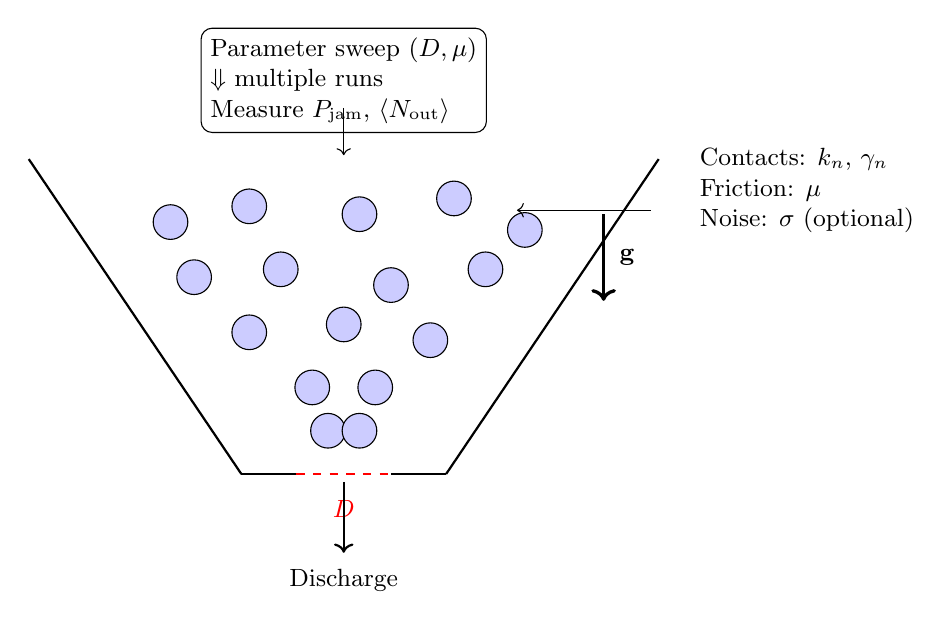
\begin{tikzpicture}[scale=1.0, every node/.style={font=\small}]
        % Funnel walls
        \draw[thick] (-4,4) -- (-1.3,0);
        \draw[thick] ( 4,4) -- ( 1.3,0);
        % Orifice
        \draw[thick] (-1.3,0) -- (-0.6,0);
        \draw[thick] ( 0.6,0) -- ( 1.3,0);
        \draw[thick, dashed, red] (-0.6,0) -- (0.6,0);
        \node[red] at (0,-0.45) {$D$};

        % Particles (schematic)
        \foreach \x/\y in {-2.2/3.2,-1.2/3.4,0.2/3.3,1.4/3.5,2.3/3.1,
                          -1.9/2.5,-0.8/2.6,0.6/2.4,1.8/2.6,
                          -1.2/1.8,0.0/1.9,1.1/1.7,
                          -0.4/1.1,0.4/1.1,
                          -0.2/0.55,0.2/0.55} {
            \draw[fill=blue!20] (\x,\y) circle (0.22);
        }

        % Gravity arrow
        \draw[->, very thick] (3.3,3.3) -- (3.3,2.2);
        \node at (3.6,2.75) {$\mathbf{g}$};

        % Contact/friction annotation
        \node[align=left, anchor=west] at (4.4,3.6) {Contacts: $k_n,\,\gamma_n$\\Friction: $\mu$\\Noise: $\sigma$ (optional)};
        \draw[->] (3.9,3.35) -- (2.2,3.35);

        % Output metrics box
        \node[draw, rounded corners, align=left] (box) at (0,5.0) {Parameter sweep $(D,\mu)$\\$\Downarrow$ multiple runs\\Measure $P_{\mathrm{jam}}$, $\langle N_{\mathrm{out}}\rangle$};
        \draw[->] (0,4.65) -- (0,4.05);

        % Discharge arrow
        \draw[->, thick] (0,-0.1) -- (0,-1.0);
        \node at (0,-1.35) {Discharge};
    \end{tikzpicture}
    \caption{{\bf Simulation workflow and geometry.} A 2D granular silo (funnel walls) discharges through an orifice of width $D$. Discs interact via dissipative normal contacts and Coulomb friction (coefficient $\mu$); optional stochastic agitation and/or mild size disorder can be added. For each $(D,\mu)$ we perform multiple realizations and compute the jam probability $P_{\mathrm{jam}}$ and discharge statistics.}
    \label{fig:selectedmethod}
\end{figure*}



\section{\label{sec:results}Results and Discussion} %%% DO NOT CHANGE!

\subsection{Effect of orifice width at fixed friction}

We first vary the orifice width $D$ while keeping the friction coefficient fixed (representative value $\mu=0.6$). Figure~\ref{fig:removed_vs_D_mu06} shows that the mean number of discharged grains $\langle N_{\mathrm{out}}\rangle$ increases strongly with $D$, transitioning from very small discharges at narrow openings to sustained flow at larger openings. Consistently, Fig.~\ref{fig:jam_vs_D_mu06} displays a sharp decrease of the jam probability with increasing $D$: for small $D$ the system jams almost surely, while above a critical range the probability drops to nearly zero within our sampling resolution.

\begin{figure}[t]
    \centering
    \includegraphics[width=\columnwidth]{md_removed_vs_D_friction_updated.png}
    \caption{{\bf Mean discharged grains vs.\ orifice width at $\mu=0.6$.} Larger openings allow more grains to exit before a stable arch forms, leading to a rapid increase of $\langle N_{\mathrm{out}}\rangle$ with $D$.}
    \label{fig:removed_vs_D_mu06}
\end{figure}

\begin{figure}[t]
    \centering
    \includegraphics[width=\columnwidth]{md_jam_vs_D_friction_updated.png}
    \caption{{\bf Jam probability vs.\ orifice width at $\mu=0.6$.} A narrow bottleneck promotes stable arch formation and yields $P_{\mathrm{jam}}\approx 1$, whereas wider openings suppress bridging and lead to $P_{\mathrm{jam}}\approx 0$ beyond a critical $D$.}
    \label{fig:jam_vs_D_mu06}
\end{figure}

\subsection{Role of disorder and stochasticity}

To probe the robustness of the clogging transition, we performed a set of runs including geometric/stochastic perturbations. Figure~\ref{fig:removed_vs_D_noise} shows that, even with added radius noise, the trend $\langle N_{\mathrm{out}}\rangle$ increases with $D$. The presence of disorder tends to reduce the likelihood of perfectly ordered packings, but does not eliminate clogging at small openings, indicating that the dominant mechanism remains frictional arch stabilization at the outlet rather than crystallization.

\begin{figure}[t]
    \centering
    \includegraphics[width=\columnwidth]{md_removed_vs_D_noise.png}
    \caption{{\bf Mean discharged grains vs.\ $D$ with radius noise.} Mild size disorder preserves the qualitative increase of discharge with $D$, suggesting that the clogging transition is controlled mainly by outlet geometry and frictional stabilization rather than by highly ordered packing.}
    \label{fig:removed_vs_D_noise}
\end{figure}

\subsection{Friction dependence for multiple outlet sizes}

We next examine how friction modifies discharge statistics at fixed $D$. Figure~\ref{fig:removed_vs_mu_multipleD} summarizes $\langle N_{\mathrm{out}}\rangle$ as a function of $\mu$ for several orifice widths. Narrow openings remain prone to clogging for essentially all friction values tested, while larger openings can sustain substantial discharge at low-to-moderate $\mu$. Increasing $\mu$ generally promotes jamming because tangential forces stabilize force chains and arches; however, the dependence can be non-monotonic in intermediate regimes where higher friction also alters packing and stress redistribution above the outlet.

\begin{figure}[t]
    \centering
    \includegraphics[width=\columnwidth]{md_removed_vs_mu_multiple_D_updated.png}
    \caption{{\bf Mean discharged grains vs.\ friction for multiple $D$.} For small $D$, the system jams quickly regardless of $\mu$. For larger $D$, moderate friction may still allow significant discharge, while high friction favors stable arches and reduces $\langle N_{\mathrm{out}}\rangle$.}
    \label{fig:removed_vs_mu_multipleD}
\end{figure}

To connect discharge statistics with the actual probability of clogging, Fig.~\ref{fig:jam_vs_mu_multipleD} reports $P_{\mathrm{jam}}(\mu)$ for the same outlet sizes. The figure highlights the combined role of geometry and friction: for sufficiently small $D$, jamming is almost guaranteed, whereas for wider openings the system remains in a free-flow regime up to relatively large $\mu$ before clogging becomes likely.

\begin{figure}[t]
    \centering
    \includegraphics[width=\columnwidth]{md_jam_vs_mu_multiple_D_updated.png}
    \caption{{\bf Jam probability vs.\ friction for multiple $D$.} Friction stabilizes arches, increasing $P_{\mathrm{jam}}$ in intermediate outlets; the largest opening remains largely unclogged within the explored $\mu$ range.}
    \label{fig:jam_vs_mu_multipleD}
\end{figure}

\subsection{Remaining particles and long-time flow interruption}

A complementary metric is the number of grains remaining in the silo after a fixed simulated time, which captures both early and late clogging. Figure~\ref{fig:remaining_vs_mu} shows a non-trivial dependence on $\mu$: at very low friction grains can rearrange and escape more easily, while at intermediate friction stable arches form more readily and more grains remain trapped. At very high friction, the system may become mechanically rigid earlier in the discharge and the remaining count saturates, consistent with a strongly jammed regime.

\begin{figure}[t]
    \centering
    \includegraphics[width=\columnwidth]{md_friction_vs_remaining.png}
    \caption{{\bf Grains remaining in the silo vs.\ friction.} The remaining population reflects the interplay between rearrangement (low $\mu$) and arch stabilization (higher $\mu$), leading to a regime where clogging is most effective at intermediate-to-high friction.}
    \label{fig:remaining_vs_mu}
\end{figure}

\subsection{Microscopic picture: arch formation at the outlet}

Finally, Fig.~\ref{fig:snapshot_mu06} shows a representative snapshot near the orifice at $\mu=0.6$ and a small opening, illustrating how a small number of grains can form a load-bearing bridge spanning the outlet. Such arches are stabilized by tangential frictional forces and by the heterogeneous force network within the granular assembly, consistent with established views of jamming and force-chain dominated mechanics in dense granular flows \cite{deGennes1999,Aranson2006,Snoeijer2003,Brodu2015}.

\begin{figure}[t]
    \centering
    \includegraphics[width=\columnwidth]{md_snapshot_mu0.6_D006.png}
    \caption{{\bf Snapshot near the outlet (example).} A stable arch forms across the orifice for $\mu=0.6$ and small $D$, blocking further discharge. The dashed lines indicate the funnel walls and the red markers highlight the outlet region.}
    \label{fig:snapshot_mu06}
\end{figure}

Overall, our results support the standard picture of clogging in bottleneck-driven granular flows: (i) increasing the outlet size rapidly suppresses jamming, and (ii) increasing friction promotes the stability of arches and force chains, thereby increasing the probability of flow interruption. While our model is two-dimensional and idealized, it captures the key qualitative trends reported across both simulations and experiments on granular discharge through constrictions \cite{Radjai2017,Zheng2024,Dauchot2010,PhysFluids2025DEMSPH}.


\section{\label{sec:conclusion}Conclusions and Outlook} %%% DO NOT CHANGE!

%%% - B6 - %%%%%%%%%%%%%%%%%%%%%%%%%%%%%%%%%%% 
%%% Customize this part: text between - B6 - and - E6 - must not appear in the final report 
\noindent
\fbox{\parbox[t][][t]{\columnwidth}{
\textbf{Points:} \fbox{\bf \textcolor{magenta}{4}} out of \textbf{44}

Here conclusions and outlook. 
}}

\textcolor{cyan}{\lipsum[1]}

\textcolor{cyan}{Lorem ipsum dolor sit amet, consectetuer adipiscing elit. Aenean commodo ligula eget dolor. Aenean massa. Cum sociis natoque penatibus et magnis dis parturient montes, nascetur ridiculus mus. Donec quam felis, ultricies nec, pellentesque eu, pretium quis, sem.  }
%%% - E6 - %%%%%%%%%%%%%%%%%%%%%%%%%%%%%%%%%%%%%%





\section{\label{sec:Contribution}Contributions} %%% DO NOT CHANGE!

%%% - B7 - %%%%%%%%%%%%%%%%%%%%%%%%%%%%%%%%%%% 
%%% Customize this part: text between - B7 - and - E7 - must not appear in the final report 
\noindent
\fbox{\parbox[t][][t]{\columnwidth}{
\textbf{Points:} \fbox{\bf \textcolor{magenta}{1}} out of \textbf{44}

Mandatory in all cases (also in the case of 1-person team). 

Add some text. See a possible example text below.
}}
Example: A.B. and C.D. conceived and implemented ... (adapt). E.F., G.H., contributed to .... etc etc. All authors ... (adapt).
%%% - E7 - %%%%%%%%%%%%%%%%%%%%%%%%%%%%%%%%%%%%%%



\section{\label{sec:COI}Conflict of Interest} %%% DO NOT CHANGE!

%%% - B8 - %%%%%%%%%%%%%%%%%%%%%%%%%%%%%%%%%%% 
%%% Customize this part: text between - B8 - and - E8 - must not appear in the final report 
\noindent
\fbox{\parbox[b][][t]{\columnwidth}{
\textbf{Points:} \fbox{\bf \textcolor{magenta}{1}} out of \textbf{44}

Add some text. See the the following Note for a clarification.
}}

{{\bf Note:} A conflict of interest can also be known as {\emph competing interest}. A conflict of interest can occur when you, or your employer, or sponsor have a financial, commercial, legal, or professional relationship with other organizations, or with the people working with them, that could influence your research.
For example check here:} \href{https://authorservices.taylorandfrancis.com/editorial-policies/competing-interest/}{https://authorservices.taylorandfrancis.com/editorial-policies/competing-interest/}
%%% - E8 - %%%%%%%%%%%%%%%%%%%%%%%%%%%%%%%%%%%%%%




\section{\label{sec:datacode}Data and Code Availability} %%% DO NOT CHANGE!

%%% - B9 - %%%%%%%%%%%%%%%%%%%%%%%%%%%%%%%%%%% 
%%% Customize this part: text between - B9 - and - E9 - must not appear in the final report 
\noindent
\fbox{\parbox[b][][t]{\columnwidth}{
\textbf{Points:} \fbox{\bf \textcolor{magenta}{1}} out of \textbf{44}

Add some text. See a possible text below.
}}

Data is available for download at ....  / can be accessed from ....

All source code and examples are made publicly available at ... . The version used in this study is archived in ... with DOI ... 
%%% - E9 - %%%%%%%%%%%%%%%%%%%%%%%%%%%%%%%%%%%%%%



%%% - B10 - %%%%%%%%%%%%%%%%%%%%%%%%%%%%%%%%%%% 
%%% Customize this part: text between - B10 - and - E10 - must not appear in the final report 
\noindent
\fbox{\parbox[b][][t]{\columnwidth}{
Score for correct amount of relevant, peer reviewed {\bf References}: 
\textbf{Points:} \fbox{\bf \textcolor{magenta}{5}} out of \textbf{44}
}}


\bibliography{biblio-FFR120-FYM119} %%% DO NOT CHANGE!
% Produces the bibliography via BibTeX.

\end{document}
